% Chapter 5

\chapter{Genome Architecture} % Main chapter title

\label{Chapter5} % For referencing the chapter elsewhere, use \ref{Chapter2} 

% \lhead{Chapter 2. \emph{Methods}} % This is for the header on each page - perhaps a shortened title

%----------------------------------------------------------------------------------------



\label{sec: Architecture}
The MVM genome is a small, non-permutated, linear, single-stranded DNA molecule \cite{pmid789912, pmid225040, Genome1, Genome2} that is \np{5085} nt in length for MVMi and \np{5149} nt for MVMp \cite{pmid3502703}. The relatively long coding sequence of approximately 4.8 kb contains two major monosense ORFs which span most of the viral genome, with some sections having overlapping coding regions \cite{pmid6298737}. The ORFs encode a non-structural (NS) gene and a structural (VP) gene and they are, by convention, termed as occupying the ``left'' or the ``right'' half of the coding sequence, respectively. The NS gene encodes four proteins that are required for the replication of the viral genome and are referred to as NS1, NS2\textsuperscript{P}, NS2\textsuperscript{Y}, as well as NS2\textsuperscript{L}. The VP gene encodes an overlapping set of capsid proteins, VP1 the minor capsid protein and VP2 the major capsid protein \cite{pmid6828378, pmid2939261, pmid2942705}. A representation of the genomic organization of MVM is illustrated in Figure~\ref{Architecture}~A, p.~\pageref{Architecture}.   

\section{The MVM Left- and Right-End Telomeres}        

The coding sequence is enclosed by short, imperfect palindromes which fold back on themselves to secondary structured duplex telomeres. Both telomeres differ considerably from each other in size, primary sequence and secondary structure \cite{pmid6298737}. Hence, they are physically and functionally dissimilar and also vary in their terminal resolution strategies at the two sites (see Section~\ref{Resolution}, p.~\pageref{Resolution}), although the molecular principles that underlie both strategies are very similar \cite{encapsidation}. 

The MVM left-end telomere is 121 nt in length and forms into a Y-shaped configuration, as depicted in Figure~\ref{Architecture}~B (left panel), p.~\pageref{Architecture}. The stem region which contains 43 base pairs (bp) is only interrupted by a mismatched bubble sequence where a triplet GAA on the inboard arm is opposed to the dinucleotide sequence GA on the outboard arm. Additionally, an asymmetric thymidine residue is located within the stem on the outboard arm in the immediate proximity to the ``ear'' that are generated by small internal palindromes. These ``ear''-like structures give rise to the Y-shaped configuration of the left-end terminus \cite{pmid225040, pmid6298737, pmid3973977, replication}. A single DNA sequence, designated the ``flip'' sequence, is conserved in the progeny viral left-end telomere, as is observed \textit{in vivo} \cite{pmid3973977}.  

The MVM right-end telomere is 248 nt in length and can be simply described as an almost perfect duplex stem structure of 121 bp (see Figure~\ref{Architecture} D, p.~\pageref{Architecture}). The palindrome is only interrupted by a triplet of unpaired nucleotides which form a small asymmetric bubble near the distal end of one strand, along with three unpaired bases which form the cross-link at the palindrome axis \cite{pmid6298737, pmid3973977}. As in homotelomeric parvoviruses, two distinct forms of the MVM right-end terminus, referred to as ``flip'' and ``flop'', are generated in equimolar amounts \textit{in vivo} (see Figure~\ref{Architecture}~D (i) and (ii), p.~\pageref{Architecture}) \cite{telomere2, encapsidation}. These two forms are the inverted complements of one another and both give rise to viral origins, called \textit{oriR} \cite{pmid1388310, pmid9765384, pmid10627544}. A small internal palindrome, surrounding the three-nt bubble, thermodynamically enables an alternative, asymmetric cruciform configuration of the right-end telomere (see Figure~\ref{Architecture}~D (iii), p.~\pageref{Architecture}) \cite{pmid6602687}. 


\subsection{Terminal Resolution \textit{versus} Asymmetric Junction Resolution}
\label{Resolution}

As is the case for most of the heterotelomeric parvoviruses, MVM shows packaging bias with minus strands preferentially encapsidated to plus strands by a 10-100-fold margin (see Section~\ref{Packaging}, p.~\pageref{Packaging}) \cite{pmid6828378, pmid3296697}. This results from differences in the efficiency of their two DNA replication origins at both ends of their genomes, rather than any strand-specific packaging sequence. In particular, the efficient nick site of the \textit{oriR} dictates the negative polarity of the packaged strand which is encapsidated in MVM virions \cite{pmid15681430}. 

In keeping with their homotelomeric counterparts, the right-end hairpin of MVM exists as an equimolar mix of flip and flop sequence orientations and is processed by a similar terminal resolution strategy. Nicking of the hairpin near the junction between palindromic and non-palindromic sequences and subsequent extension of the right-end terminus allows an efficient inversion of the palindrome (see step iii and iv in Figure~\ref{RHR}, p.~\pageref{RHR}). On the contrary, the MVM left-end hairpin predominates in the flip orientation, indicating its generation by an asymmetric junction resolution mechanism \cite{pmid12743281}. Briefly, the asymmetric bubble sequence in the stem of the MVM left-end telomere (see Figure~\ref{Architecture}~B, p.~\pageref{Architecture}) prevents assembly of an active nicking complex. Thus, the left-end telomere cannot function as a replication origin in its hairpin conformation \cite{pmid8995615}. During rolling hairpin replication (RHR) (see Section~\ref{Replication}, p.~\pageref{Replication}), the hairpin is unfolded, extended, and copied to form the fully base-paired, imperfect palindromic junction sequence that bridges adjacent genomes in an intermediate dimer replicative form (dRF) (see Figure~\ref{Architecture}~B (right panel), p.~\pageref{Architecture}). It was demonstrated that such junctions can initiate DNA replication in a NS1-dependent manner \cite{pmid8076610, pmid1530771}. Formation of the dimer junction effectively segregates two potential origins of DNA replication, one derived from each arm of the hairpin, on either side of the junction's symmetry axis but only one of these origins is active. The activity is regulated by the sequence of the asymmetric bubble which serves as a precise spacer between the NS1 binding site and the parvovirus initiation factor (PIF). Binding of PIF stabilizes the interaction of NS1 with the active (TC) origin (\textit{OriL\textsubscript{TC}}) but not with the inactive (GAA) origin (\textit{OriL\textsubscript{GAA}}) \cite{pmid11435581}. The minimal left-end origin of replication is called \textit{oriL} and shown in Figure~\ref{Architecture}~C, p.~\pageref{Architecture}. It extends from two 5'-ACGT-3' motifs which represent binding sites for PIF \cite{pmid8995666, pmid9223459, pmid10523663}, to a 5'-(ACCA)\textsubscript{2}-3' binding site for the viral initiator nickase NS1 \cite{pmid7853501}, and finally to the active nick site \cite{pmid8076610}. Recent studies have revealed that MVM tolerates both sequence and orientation changes in its left-end hairpin. In which case it can be deduced that maintaining the flip orientation of the left-end telomere is a consequence of, but not the reason for, asymmetric dimer junction resolution. However, the same study indicated that asymmetric left-end processing is crucial for MVM replication \cite{pmid22933276}.  

In summary, the heterotelomeric hairpins, along with a few adjacent nucleotides, provide all of the \textit{cis}-acting information required for efficient genome replication and encapsidation. In particular, these terminal nucleotides, representing less than 10~\% of the entire genome, create the replication origins by providing nicking sites that are used as a primer for DNA synthesis and to effectively separate unit-length genomes for DNA packaging. Additionally, they function as flexible hinge regions used to establish and re-orient the replication fork, allowing it to roll back and forth along the linear viral DNA \cite{telomere2, telomere3, handbook, RHR}.        

\section{Genetic variability}

When compared with cellular DNA, the genome of MVM has a relatively high GC-content (42~\%) \cite{pmid6298737}, partially reflecting its high density of regulatory elements \cite{telomere}. The complexity of the viral genome is increased by transcriptional promoter sequences and various splicing signals that are embedded within the same primary sequence, beyond the encoded proteins which are organized in multiple overlapping ORFs. Following inoculation of clonal populations of MVMi stocks in mice, genetically different antibody-escape variants emerged \textit{in vivo}. This indicates that viral replication appears to support the generation of heterogeneity \cite{pmid12552010}. The best studied example is represented by the emergent branch of CPV which evolved from FPV in 1978 allowing the virus to expand its host range to canines. The substitution rate of CPV resembles that seen in rapidly evolving RNA viruses, as for example HIV-1 and human influenza A virus \cite{pmid15626758}. Remarkably, such diversity occurred despite the fact that the viral genome is replicated using a subset of the host's DNA replication machinery \cite{pmid8614999, pmid10792046}. Hence, the mutation rates would be expected to be low \cite{pmid15964835, pmid19540301}. Probably, the unidirectional strand-displacement mechanism may exhibit lower fidelity compared to the bidirectional replication of eukaryotic genes. Additionally, the concatemeric duplex intermediates may allow for inter- and intramolecular recombination during replication of the viral DNA \cite{telomere}. Moreover, there are several lines of evidence that MVM exploits the DNA damage response machinery early in infection in order to enhance its replication and to improve virus-induced cell cycle arrest in the S-phase \cite{pmid20949077}. Therefore, it seems possible that under such conditions the replication forks may be more error-prone. Finally, environmentally induced changes in the viral DNA sequence, such as depurination or deamination, cannot be corrected because virions contain ssDNA and hence do not provide a template for excision or mismatch repair systems. Nonetheless, the genetic complexity, a consequence of the constrained genome size, severely and selectively restricts the types of tolerated modifications \cite{telomere}.   

\begin{figure}
\centering
  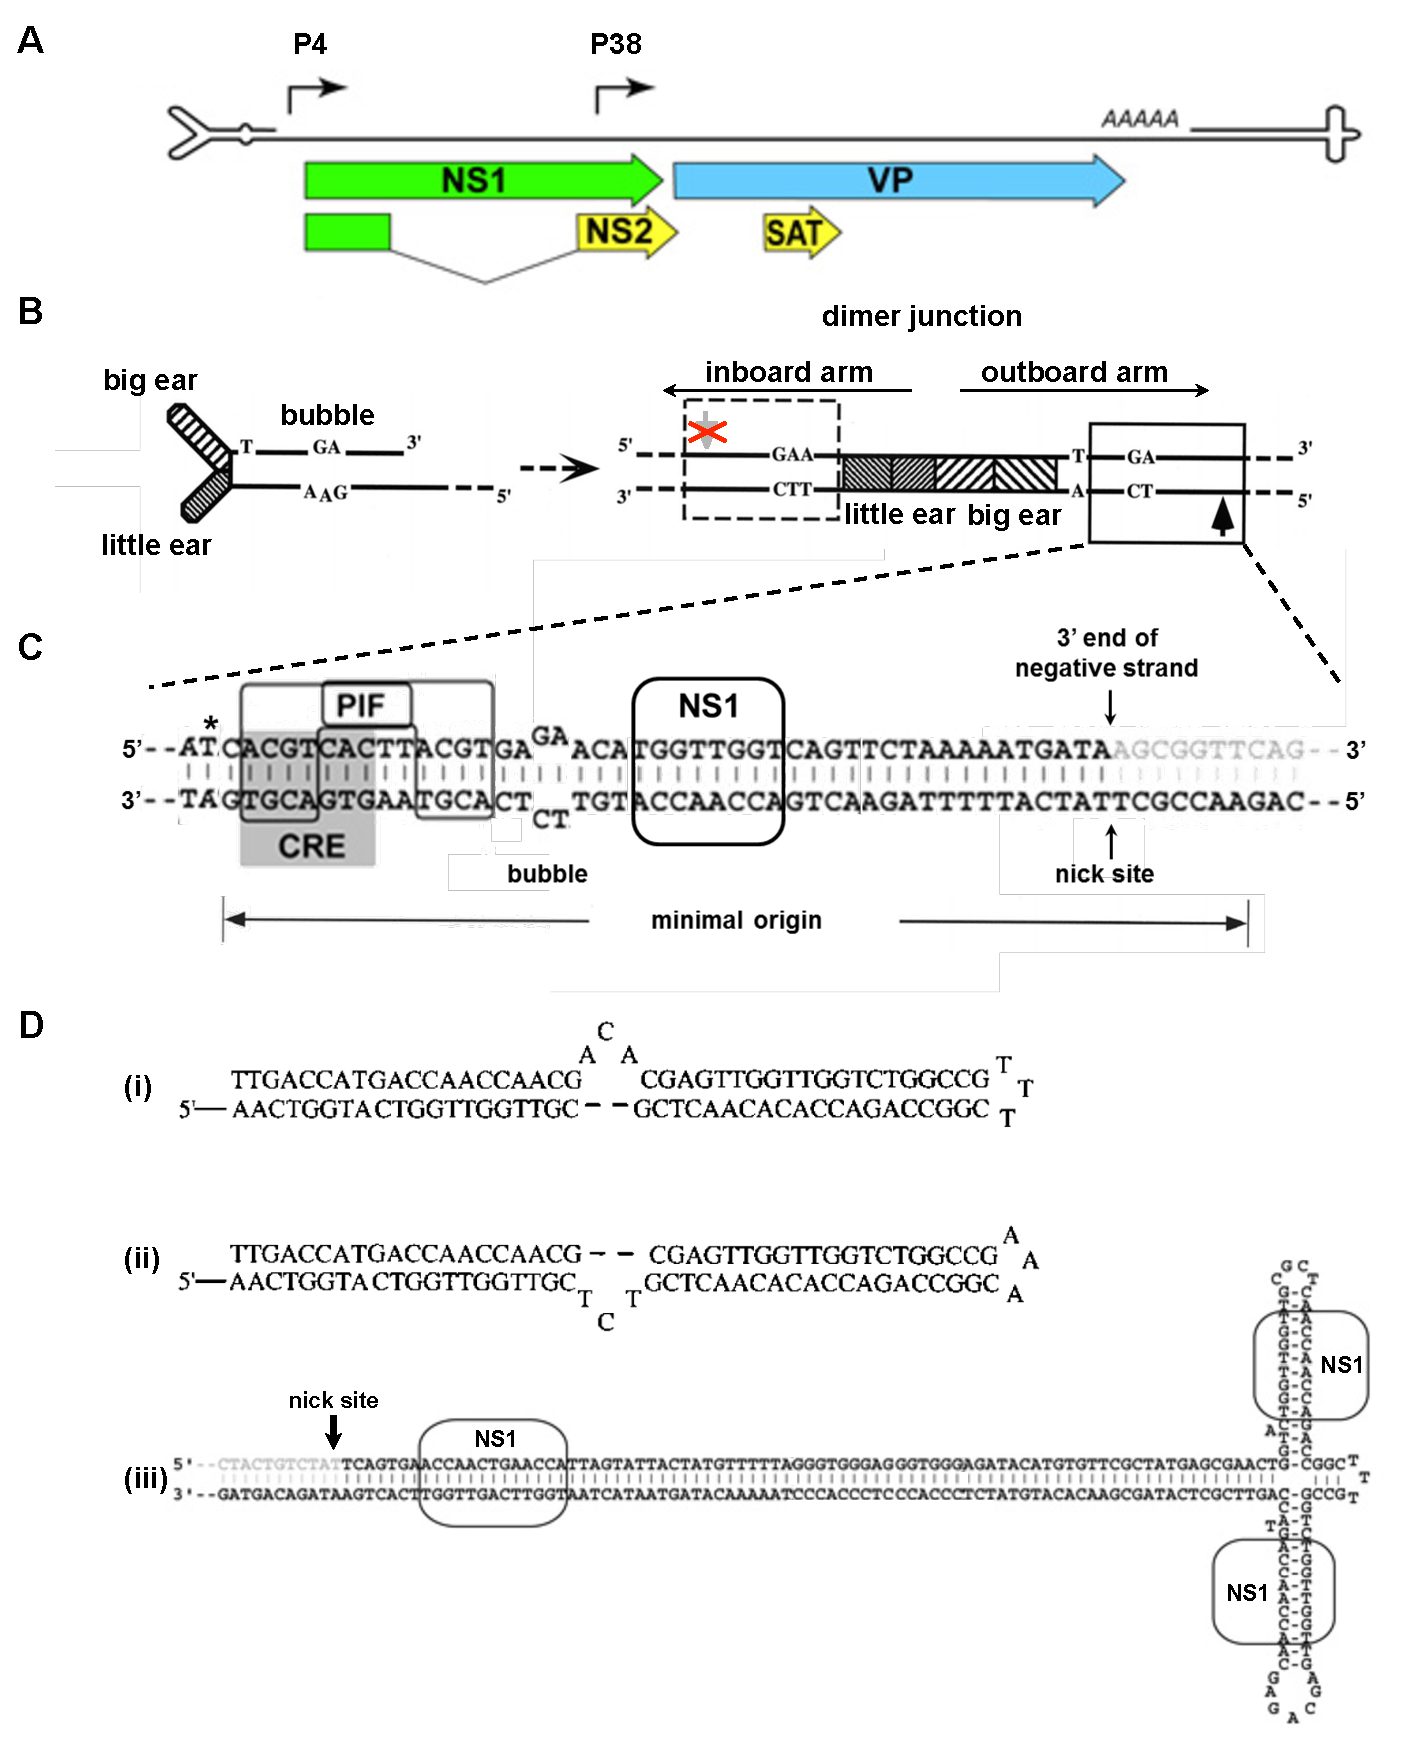
\includegraphics[scale=0.55]{Architecture}
  \caption[Genome architecture of MVM]
   {Genome architecture of MVM. \textbf{(A)} Schematic of the predicted structures of the terminal hairpins, scaled approximately 20$\times$ relative to the rest of the genome. Major ORFs are represented by arrowed boxes and alternative RNA splicing for NS2 is indicated. Proteins are shaded green for the major replication initiator protein (NS1), blue for the structural (VP) proteins of the capsid, and yellow for sequences unique to the ancillary NS proteins. The two transcriptional promoters, P4 and P38, are indicated by rightward arrows and the polyadenylation site by the AAAAA-sequence block \cite{small}. \textbf{(B)} Diagram of the left-end hairpin of MVM and its dimer junction. Asymmetries, such as the ``ear''-like structures, extra-helical T, and bubble sequence are indicated. The duplex, dimer junction, generated by RHR (see Section~\ref{Replication}, p.~\pageref{Replication}), is shown on the right hand side. The short, palindromic sequences derived from the hairpin ears are represented by cross-hatched boxes. The active \textit{OriL\textsubscript{TC}} is boxed, with an arrow indicating the nick site. The equivalent sequence generated on the GAA side of the bubble is framed by a dashed box with an arrow at the potential nick site that is crossed out to indicate that \textit{OriL\textsubscript{GAA}} is not active \cite{pmid12885883, pmid16928767}. \textbf{(C)} Sequence details of the active left-end origin (approx. 50 bp) are shown, with an arrow indicating the active nick site. The minimal sequence required for origin activity is indicated by the double-headed arrow. Sequences of the bubble and the PIF, cAMP-responsive element (CRE), and NS1 binding sites are indicated. An asterisk represents the position of the extra-helical T, now base paired, and the gray box below it indicates the CRE consensus sequence \cite{pmid12885883}. \textbf{(D)} Alternate conformations of the right-end hairpin sequences of MVM. The right-end terminus can form a hairpin structure in either the flip (i) of flop (ii) sequence orientation or a cruciform structure (iii). In the cruciform configuration, the binding sites for the replicator protein, NS1, are boxed and their site of nucleolytic cleavage is represented by a vertical arrow \cite{pmid8614999}.
} 
\label{Architecture}
\end{figure}


\nomenclature{VP}{Viral protein}
\nomenclature{NS}{Non-structural (protein)}
\nomenclature{PIF}{Parvovirus initiation factor}
\nomenclature{CRE}{cAMP-responsive element}
\nomenclature{SAT}{Small alternatively translated protein}